\documentclass[a4paper, 12pt]{report}
\usepackage[utf8]{inputenc}
\usepackage[french]{babel}
\usepackage{graphicx}
\usepackage{hyperref}
\usepackage{url}
\usepackage{amsmath}
\usepackage{listings}

\begin{document}

    \hypersetup{pdfborder=0 0 0}

    \setcounter{page}{0}

    \begin{minipage}{0.6\linewidth}
        \textbf{Université de Caen Normandie}\\
        U.F.R. Sciences \\
        Département Informatique\\
        Année 2020-2021
    \end{minipage}

    \begin{minipage}{0.5\linewidth}
        \begin{flushright}
            
\includegraphics[scale=1.2]{images/logo.png}
        \end{flushright}
    \end{minipage}

    \vspace{5cm}

    \begin{center}
        \huge \textbf{PROJET BATAILLE NAVALE}\\
    \end{center}

    \vspace{2cm}

    \textbf{Réalisé par :} \\
    Ben Kabongo Buzangu\\
    Martin Jules\\
    Mamadou Mouctar Bah\\
    Meryam El Boudouti\\

    \newpage
    \chapter*{Introduction}
    Dans le cadre du cours de Complément POO, il a été demandé aux étudiants de la L2 Informatique de réaliser en groupe
    un projet informatique de bout en bout afin de parfaire leur savoir-faire et leurs compétences en travaux d'équipes.

    Il s'agit ici de réaliser un jeu de \textbf{Bataille navale}, en utilisant le langage \textbf{Java} et sa
    bibliothèque intégrée \textbf{Swing}. La version du langage utilisée pour le projet est la 1.8.

    Le patron d'architecture utilisé pour la conception de l'application est le \textbf{MVC} pour \textbf{Modèle - Vue -
    Contrôleur}. Nous avons commencé par implémenter le modèle avec les éléments nécessaires ainsi que la logique du jeu.
    Ensuite, nous avons conçu la partie vue-contrôleur en rajoutant une interface graphique.

    Dans la suite de ce rapport, nous allons vous présenter cette conception et en expliquer les éléments constitutifs.

    \chapter{Diagramme des classes}
    \begin{figure}[h!]
        \centering
        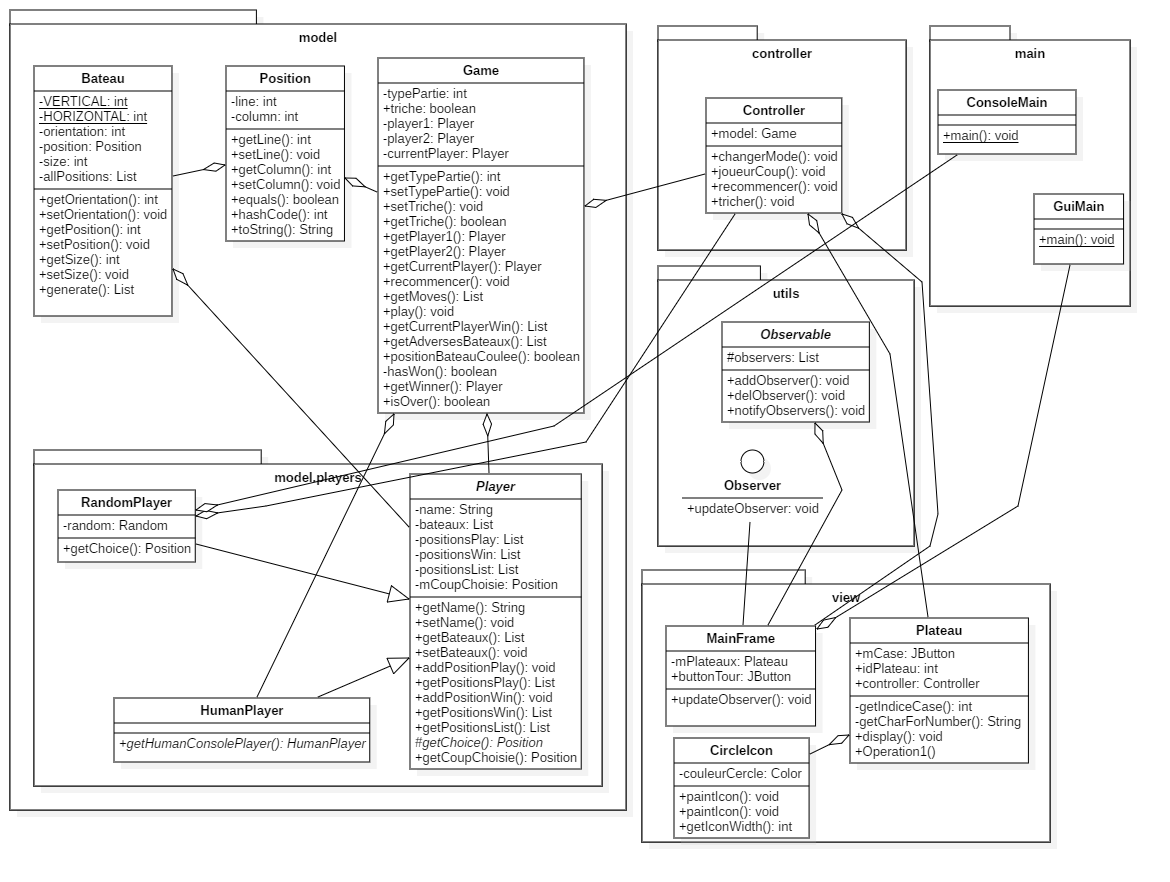
\includegraphics[scale=0.4]{images/diagrammeClasse.png}
        \caption{Diagramme des classes}
        \label{fig:diagramme_classes_illustration}
    \end{figure}


    \chapter{Modèle de l'application}
    Le modèle de l'application comprend les éléments constitutifs d'un jeu de bataille navale et la logique de ce dernier.

    \section{Gestion de la position}
    La notion de position est importante dans un jeu de bataille navale. La flotte des joueurs est donnée par une matrice
    à deux dimensions. Un joueur choisira donc systématiquement une position dans la flotte adverse sur laquelle tirer.
    Le tir est soit réussi si un pion du joueur adverse est touché ; soit un échec si aucun pion du joueur adverse n'est
    touché. Il a donc été nécessaire de mettre en place un mécanisme de gestion de positions. \\

    Nous avons donc créé la classe \textbf{model.Position} afin de représenter une position. Une position est la donnée
    d'un numéro de ligne entre 0 et 9 et d'un numéro de colonne entre 0 et 9.
    Deux positions sont égales si leurs numéros de ligne et de colonne sont respectivement égales

    \section{Les joueurs}
    La bataille navale est un jeu dans lequel s'affrontent deux joueurs. Pour chacun, une certaine quantité d'informations
    importantes est à retenir afin de faire évoluer les parties de jeu. \\

    Nous avons créé le package \textbf{model.players} afin de représenter les joueurs. La classe mère de toutes les
    classes de joueurs est la classe \textbf{model.players.Player}.

    Chaque joueur sera initialisé par un nom et par une liste de bateaux.

    Nous sauvegardons dans trois liste de positions importantes pour chaque joueur.\\
    \textbf{La liste des positions occupées} contient toutes les positions occupées par le joueur dans sa propre flotte.\\
    \textbf{La liste de positions jouées} contient toutes les positions que le joueur a jouée pour la flotte adverse.
    Cela évite à ce dernier de sélectionner des positions déjà jouées. \\
    \textbf{La liste des positions gagnées} contient toutes les positions auxquelles le joueur a touché le joueur adverse.\\

    Nous nous sommes assurées de représenter dans chacune des listes chaque position une et une seule fois. Ainsi, on
    conclura qu'un joueur a gagné une partie si la taille de la liste des positions gagnées est égale à la taille de la
    liste des positions occupées du joueur adverse. \\

    Afin de pouvoir initialiser différents types de jeux, nous avons créé deux types de joueurs : le joueur humain
    (\textbf{model.players.HumanPlayer}) et le joueur aléatoire (\textbf{model.players.RandomPlayer}). Le joueur humain
    choisit lui-même les positions où jouer ; pour le joueur aléatoire, ces positions sont choisies aléatoirement.

    \section{Les bateaux}
    Dans un jeu de bataille navale, chaque joueur repartit ses bateaux sur différentes positions de la flotte. Nous
    avons opté pour une repartition aléatoire, pour tous les types de joueurs.
    Les bateaux possèdent une taille, une orientation et une liste de positions adjacentes.
    Nous avons implémenté la notion de bateaux dans la classe \textbf{model.Bateau}.

    \section{Gestionnaire de partie}
    Afin de gérer les parties en cours, nous avons créé la classe \textbf{model.Game}. Elle prend en paramètre deux
    joueurs, gère le tour de chacun et effectue les mises à jour adéquates des différentes listes de positions des
    joueurs au fur et à mesure du jeu.

    C'est la classe observable de notre modèle. Elle renseigne ses observateurs des changements qui surgissent au cours
    d'une partie lancée, du début à la fin de cette dernière.

    \section{Mise en place du pattern observateur}
    Le pattern observateur fait parti de la démarche MVC. La classe \textbf{Game} représente la classe modèle de notre
    application. Elle hérite de la classe \textbf{utils.Observable}. Les classe implémentant l'interface
    \textbf{utils.Observer} peuvent donc observer une partie en cours et être mises au courant des mises à jour.
    La vue de notre interface graphique implémente cette interface.

    \section{Jeu en console}
    Nous avons créé une version console du jeu, accesible à partir de \textbf{main.ConsoleMain}.
    \begin{figure}[h!]
        \centering
        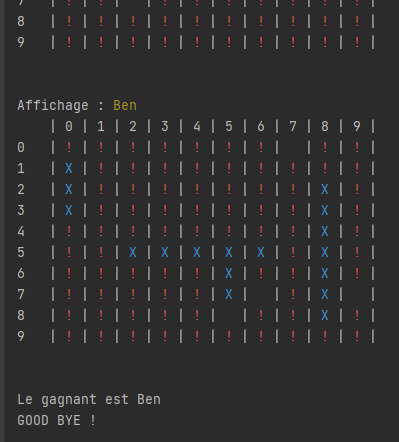
\includegraphics[scale=0.5]{images/console.png}
        \caption{Jeu console}
        \label{fig:jeu_console_illustration}
    \end{figure}


    \chapter{Interface graphique}
    L'interface graphique de notre application a été implémentée dans le package \textbf{view}.
    La classe de base \textbf{MainFrame} implémente l'interface \textbf{utils.Observer}. Au fur à mesure des coups
    de chaque joueur, l'interface est mise à jour. \\

    Trois modes de jeu ont été implémentés : le mode huamin contre joueur aléatoire, le mode avec deux joueurs aléatoires
    et le mode avec des joueurs humains.

    \begin{figure}[h!]
        \centering
        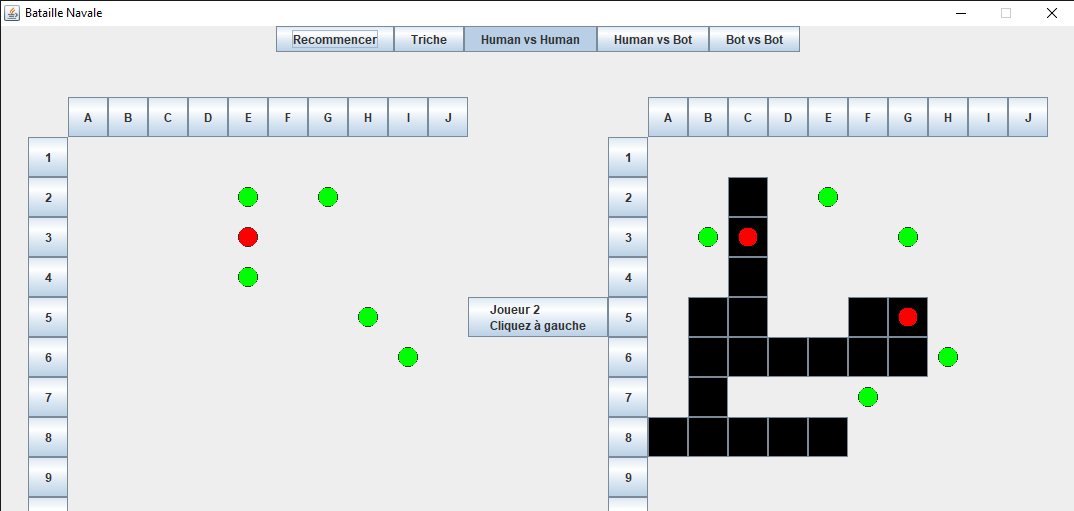
\includegraphics[scale=0.4]{images/gui.png}
        \caption{Interface graphique}
        \label{fig:interface_graphique_illustration}
    \end{figure}
\end{document}